\documentclass[12pt]{article}
\usepackage[utf8]{inputenc}
\usepackage[russian]{babel}
\usepackage{graphicx}
\usepackage{subcaption}
\graphicspath{ {./images/} }


\begin{document}

Дубровских Никита 221-361

\textit{\textbf{Вариант 7}}

\textit{\textbf{Задание 14.}}

\textit{Торговая компания имеет филиалы в 8 точках города. Транспортная
сеть с указанием расстояний в километрах представлена на рис. Определить
кратчайшие пути между узлом 1 и всеми остальными узлами транспортной
сети.}

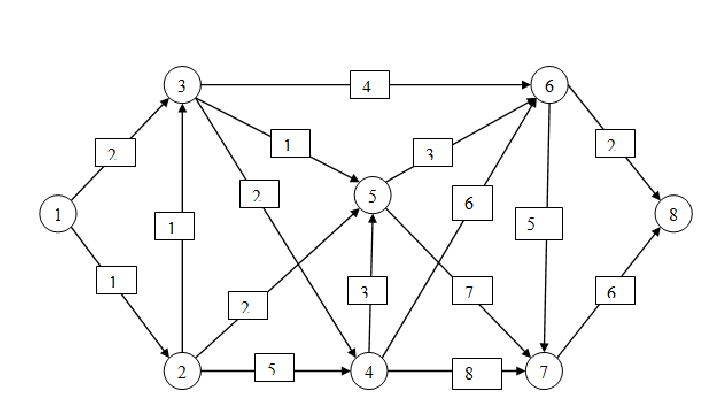
\includegraphics[width=350]{14_task.png}

\underline{Решение:}

\begin{center}
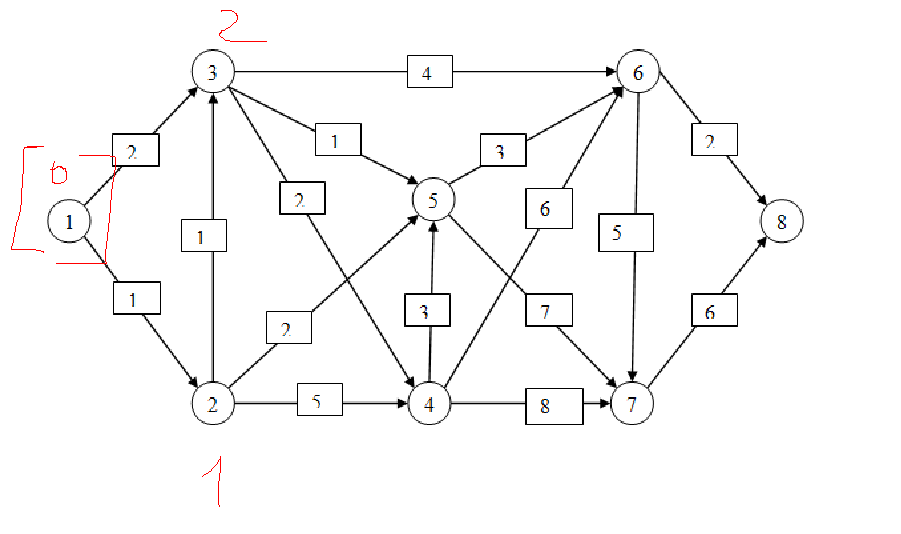
\includegraphics[width=350]{14_1.png}
\end{center}
\begin{center}
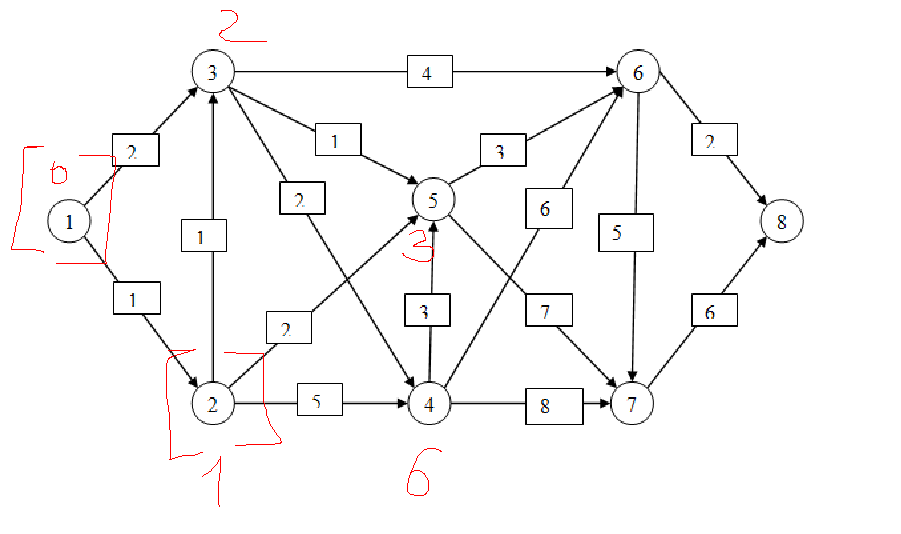
\includegraphics[width=350]{14_2.png}
\end{center}
\begin{center}
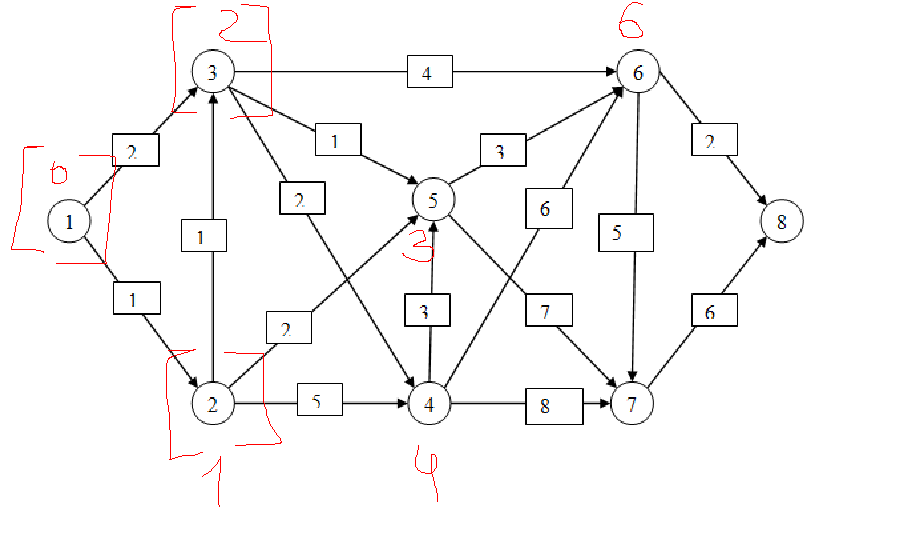
\includegraphics[width=350]{14_3.png}
\end{center}
\begin{center}
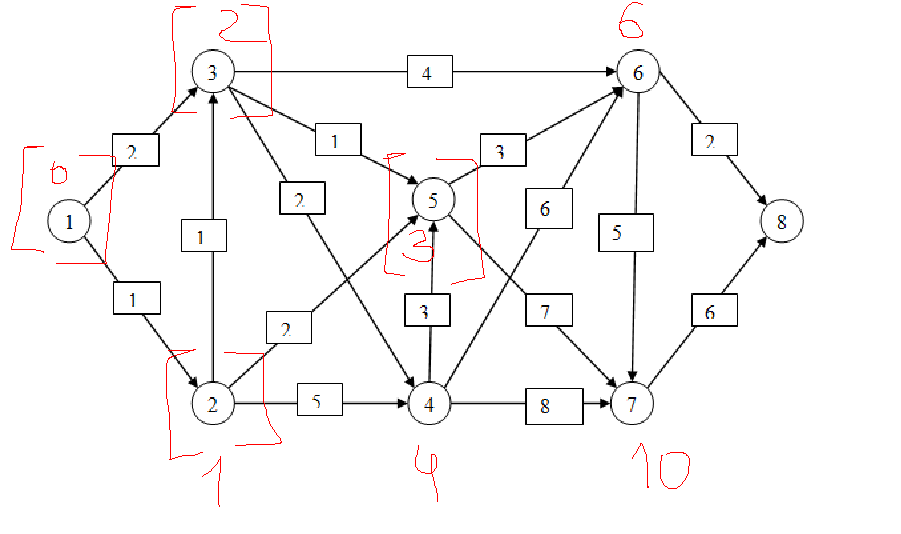
\includegraphics[width=350]{14_4.png}
\end{center}
\begin{center}
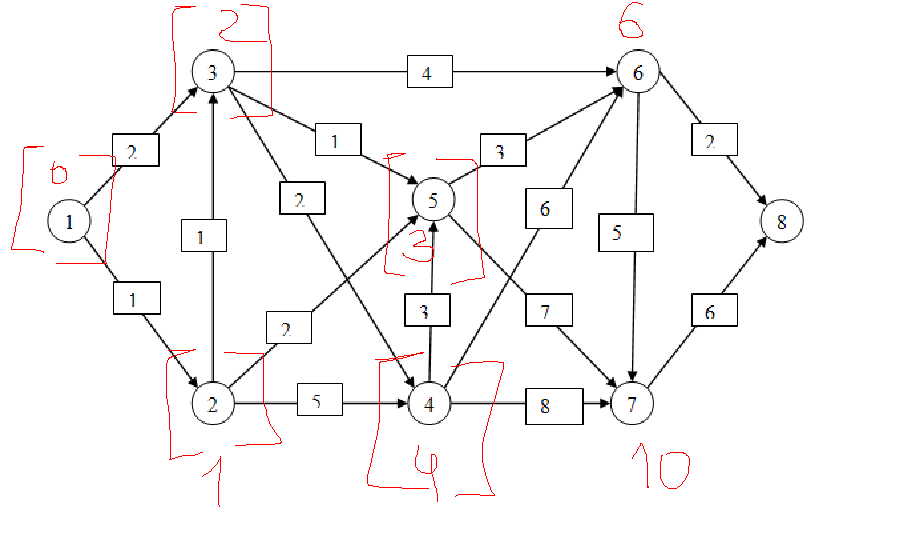
\includegraphics[width=350]{14_5.png}
\end{center}
\begin{center}
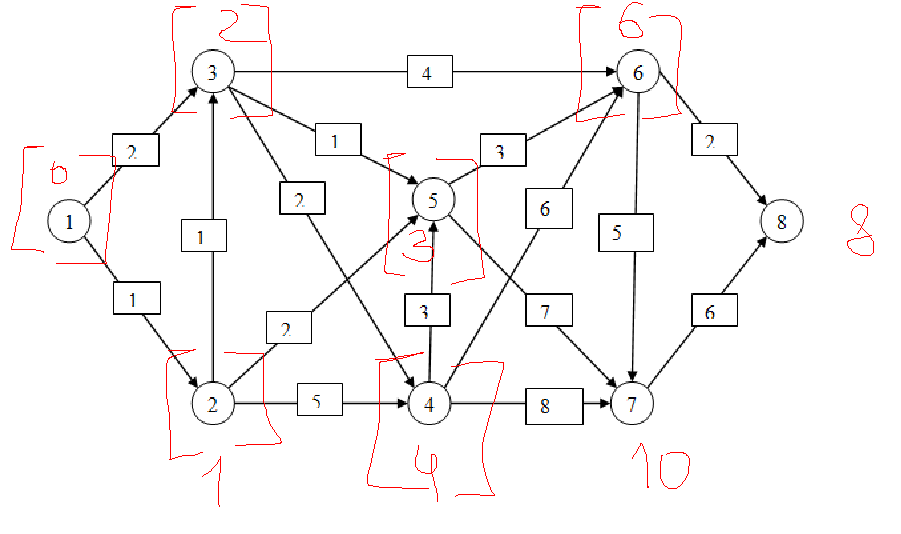
\includegraphics[width=350]{14_6.png}
\end{center}
\begin{center}
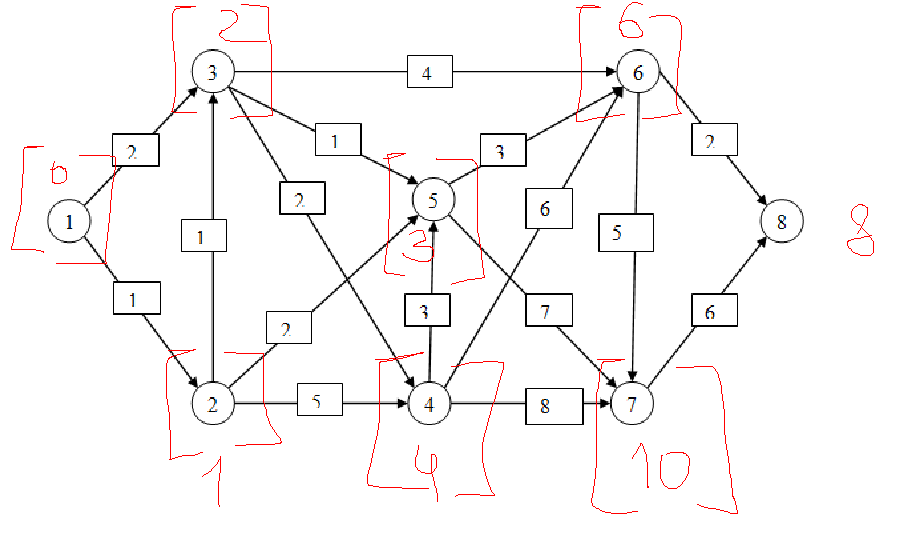
\includegraphics[width=350]{14_7.png}
\end{center}
\begin{center}
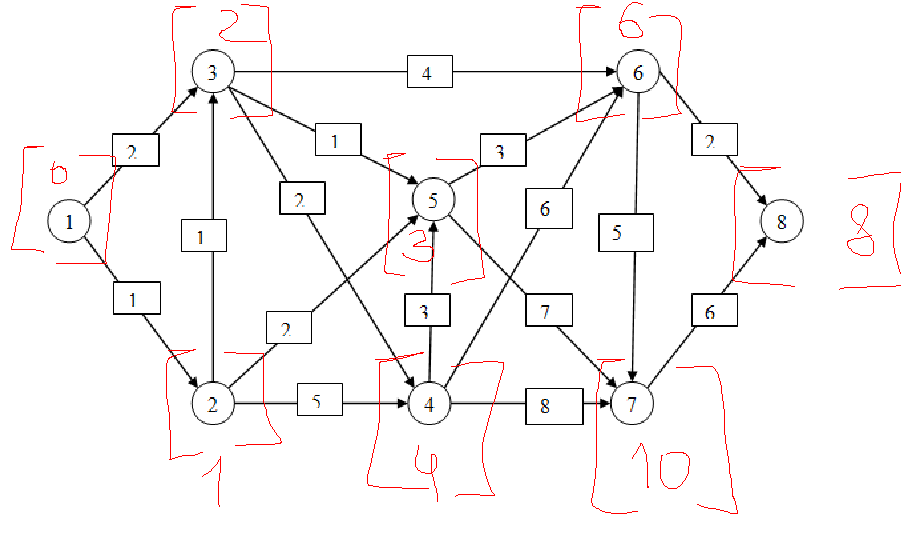
\includegraphics[width=350]{14_8.png}
\end{center}

Таким образом, кратчайшие пути из вершины 1: (0,1,2,4,3,6,10,8).

\end{document}
